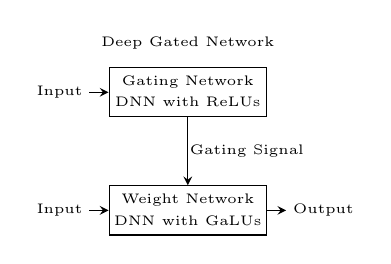
\begin{tikzpicture}

\node []  (fntext)at (5,1+0.25) {\tiny{Deep Gated Network}};
%Feature Network
\node [draw,
	minimum width=2cm,
	minimum height=0.625cm,
]  (fnbox)at (5,0.375+0.25) {};
\node []  (fntext)at (5,0.5+0.25) {\tiny{Gating Network}};

\node []  (fntext)at (5,0.25+0.25) {\tiny{DNN with ReLUs}};


%Feature Network Input
\node (fin) [left of=fnbox,node distance=1.25cm, coordinate] {};
\node[left=-1pt] at (fin.west){\tiny{Input}};
\draw[-stealth] (fin.center) -- (fnbox.west);




%Value Network

\node [draw,
	minimum width=2cm,
	minimum height=0.625cm,
]  (vnbox)at (5,-0.875) {};
\node []  (fntext)at (5,-0.75) {\tiny{Weight Network}};
\node []  (vntext)at (5,-1) {\tiny{DNN with GaLUs}};

%Value Network Input
\node (vin) [left of=vnbox,node distance=1.25cm, coordinate] {};
\node[left=-1pt] at (vin.west){\tiny{Input}};
\draw[-stealth] (vin.center) -- (vnbox.west);

%Feature Network Output
\node (vout) [right of=vnbox,node distance=1.25cm, coordinate] {};
\node[right=-1pt] at (vout.west){\tiny{Output}};
\draw[-stealth]  (vnbox.east)--(vout.center);



\draw[-stealth]  (fnbox.south)--(vnbox.north);

\node []  (gates)at (5.75,-0.125) {\tiny{Gating Signal}};


\end{tikzpicture}

